%%% LaTeX Template: Designer's CV
%%%
%%% Source: http://www.howtotex.com/
%%% Feel free to distribute this template, but please keep the referal to HowToTeX.com.
%%% Date: March 2012


%%%%%%%%%%%%%%%%%%%%%%%%%%%%%%%%%%%%%
% Document properties and packages
%%%%%%%%%%%%%%%%%%%%%%%%%%%%%%%%%%%%%
\documentclass[a4paper,12pt,final]{memoir}

% misc
\renewcommand{\familydefault}{bch}	% font
\pagestyle{empty}					% no pagenumbering
\setlength{\parindent}{0pt}			% no paragraph indentation


% required packages (add your own)
\usepackage{flowfram}										% column layout
\usepackage[top=1cm,left=1cm,right=1cm,bottom=1cm]{geometry}% margins
\usepackage{graphicx}										% figures
\usepackage{url}
\usepackage{hyperref}										% URLs
\usepackage[usenames,dvipsnames]{xcolor}					% color
\usepackage{multicol}										% columns env.
	\setlength{\multicolsep}{0pt}
\usepackage{paralist}										% compact lists
\usepackage{tikz}

\definecolor{light-gray}{gray}{0.3}
\hyphenation{in-terested}

%%%%%%%%%%%%%%%%%%%%%%%%%%%%%%%%%%%%%
% Create column layout
%%%%%%%%%%%%%%%%%%%%%%%%%%%%%%%%%%%%%
% define length commands
\setlength{\vcolumnsep}{\baselineskip}
\setlength{\columnsep}{\vcolumnsep}

% frame setup (flowfram package)
% left frame
\newflowframe{0.35\textwidth}{\textheight}{0pt}{0pt}[left]
	\newlength{\LeftMainSep}
	\setlength{\LeftMainSep}{0.35\textwidth}
	\addtolength{\LeftMainSep}{1\columnsep}

% small static frame for the vertical line
\newstaticframe{1.5pt}{\textheight}{\LeftMainSep}{0pt}

% content of the static frame
\begin{staticcontents}{1}
\hfill
\tikz{%
	\draw[loosely dotted,color=MidnightBlue,line width=1.5pt,yshift=0]
	(0,0) -- (0,\textheight);}%
\hfill\mbox{}
\end{staticcontents}

% right frame
\addtolength{\LeftMainSep}{1.5pt}
\addtolength{\LeftMainSep}{1\columnsep}
\newflowframe{0.6\textwidth}{\textheight}{\LeftMainSep}{0pt}[main01]


%%%%%%%%%%%%%%%%%%%%%%%%%%%%%%%%%%%%%
% define macros (for convience)
%%%%%%%%%%%%%%%%%%%%%%%%%%%%%%%%%%%%%
\newcommand{\Sep}{\vspace{1.5em}}
\newcommand{\SmallSep}{\vspace{0.5em}}

\newenvironment{AboutMe}
	{\ignorespaces}
	{\Sep\ignorespacesafterend}

\newcommand{\CVSection}[1]
	{\Large\textbf{#1}\par
	\SmallSep\normalsize\normalfont}

\newcommand{\CVItem}[1]
	{\textbf{\color{MidnightBlue} #1}}


%%%%%%%%%%%%%%%%%%%%%%%%%%%%%%%%%%%%%
% Begin document
%%%%%%%%%%%%%%%%%%%%%%%%%%%%%%%%%%%%%
\begin{document}

% Left frame
%%%%%%%%%%%%%%%%%%%%
\begin{figure}
	\hfill
	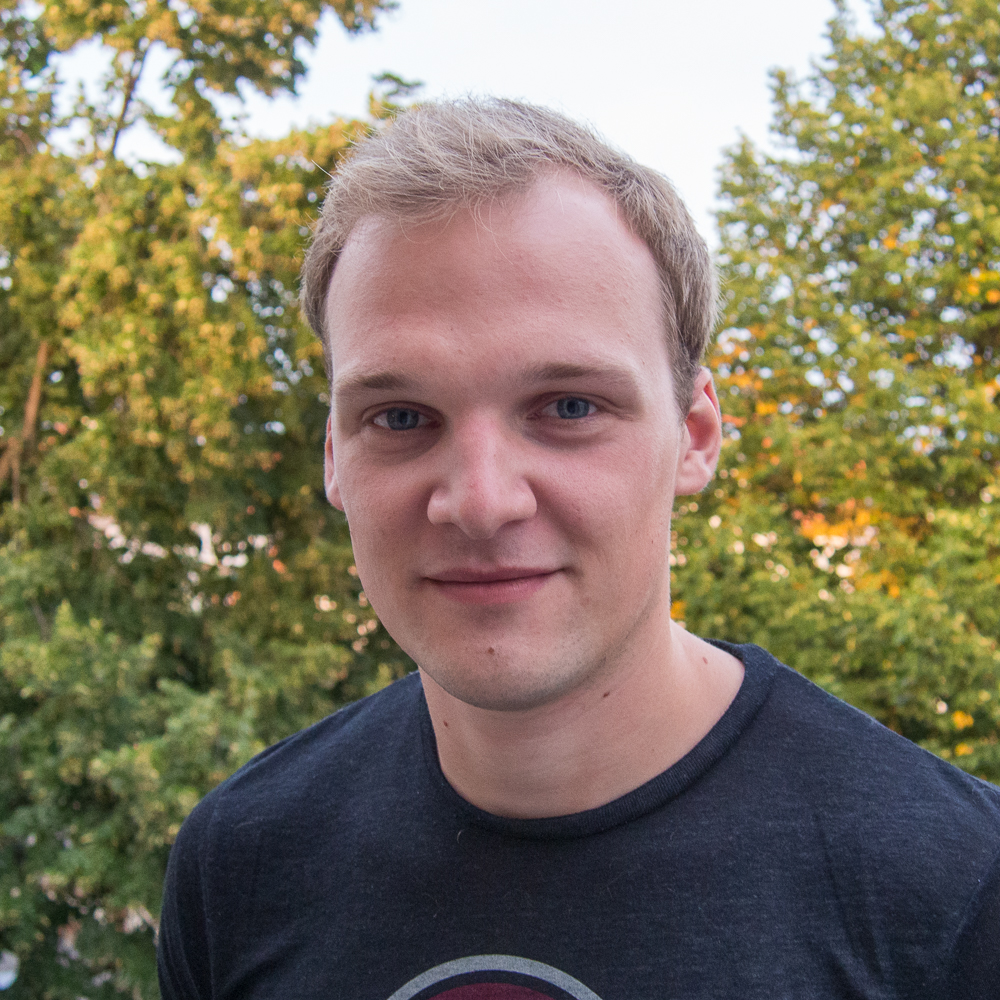
\includegraphics[width=\columnwidth]{igor.jpg}
	\vspace{-5cm}
\end{figure}

\begin{flushleft}\small
	\textbf{Name:} Bogoslavskyi Igor\\
	\SmallSep
	\textbf{Nationality:} Ukrainian\\
	\SmallSep
	\textbf{Phone:} Upon request \\
	\SmallSep
	\textbf{Address:} Upon request \\
	\Sep
	\textbf{On the Web:}\\
	\SmallSep
	\href{mailto:igor.bogoslavskyi@gmail.com}{igor.bogoslavskyi@gmail.com}\\
	\SmallSep
	\href{https://de.linkedin.com/in/igor-bogoslavskyi-72650b43}{LinkedIn::Igor Bogoslavskyi}\\
	\SmallSep
	\href{https://github.com/niosus}{GitHub::niosus}\\
	\SmallSep
	\textbf{University website:}\\
	\SmallSep
	\url{http://www.ipb.uni-bonn.de/people/igor-bogoslavskyi/}\\
\end{flushleft}
\normalsize

\framebreak{}


% Right frame
%%%%%%%%%%%%%%%%%%%%
\Huge\bfseries {\color{MidnightBlue}Dr.~Igor Bogoslavskyi} \\
\Large\bfseries  Post-doctoral Researcher \\

\normalsize\normalfont{}

% About me
\begin{AboutMe}
I am a researcher at the lab for photogrammetry and robotics at the University
of Bonn led by Prof.~Dr.~Cyrill Stachniss, where I have received my PhD in 2018.
Before moving to Bonn, I have finished my Master of Science studies at the
University of Freiburg in Germany in 2011 at the AIS laboratory led by
Prof.~Dr.~Wolfram Burgard, and Bachelor of Science in Applied Maths in Ukraine
in 2007. My current interests lie in scene interpretation, perception, mapping
and navigation for mobile robots. I am also passionate about code and maintain a
couple of open source projects in C++ and Python that can be found on my GitHub.
\end{AboutMe}

% Experience
\CVSection{Work Experience}
\CVItem{2014 --- Present, Researcher, Photogrammetry Lab
\newline Rheinische Friedrich-Wilhelms University Bonn, Germany}
\newline
I am a researcher at the University of Bonn at the Photogrammetry and Robotics
lab. My advisor is Prof.~Dr.~Cyrill Stachniss. For a list of all my projects and
publications during this time please see the next page.
\SmallSep{}

\CVItem{2017, Robotics Software Engineering Intern
\newline \href{https://nuro.ai/}{Nuro}, Mountain View, USA}
\begin{compactitem}[\color{MidnightBlue}$\circ$]
\item Worked in perception team on an autonomous delivery bot.
\item LiDAR scene interpretation, sensor calibration.
\end{compactitem}

\CVItem{2012 --- 2014, Research Assistant, AIS Lab
\newline Albert Ludwigs University of Freiburg, Germany}
\begin{compactitem}[\color{RoyalBlue}$\circ$]
\item Worked with ASUS Xtion mounted onto various platforms.
\item Implemented traversability analysis for a mobile robot as part of ROVINA
project.
\item Results published at ECMR'13.
\end{compactitem}
\SmallSep{}

\CVItem{2012 --- 2013, Research Assistant, HRL Lab
\newline Albert Ludwigs University of Freiburg, Germany}
\begin{compactitem}[\color{RoyalBlue}$\circ$]
	\item Worked with a Kinect sensor mounted onto the NAO robot.
	\item Implemented a system that detected human pointing gestures generating a
	goal for a robot to go to.
\end{compactitem}
\SmallSep

\CVItem{2011 --- 2012, Tutor, Image Processing Course
\newline Albert Ludwigs University of Freiburg, Germany}
\begin{compactitem}[\color{RoyalBlue}$\circ$]
\item Worked as a TA during the first semester of my masters.
\item Helped students to accomplish Computer Vision programming assignments.
\end{compactitem}
\SmallSep

\CVItem{2010 --- 2011, Junior Software Engineer
\newline Timecode LLC, Kyiv, Ukraine}
\begin{compactitem}[\color{RoyalBlue}$\circ$]
\item Android game programming.
\item Store for ASUS Xtion written in C\#.
\end{compactitem}

\SmallSep
\framebreak
\clearpage
\framebreak{}
	% LEFT FRAME 2nd PAGE
	\SmallSep{}
	\vspace{-2mm}

	\CVSection{I Mostly Code In}
	\begin{compactitem}[\color{MidnightBlue}$\circ$]
		\item C\texttt{++}
		\item Python
		\item Java
		\item Matlab/Octave
	\end{compactitem}
	\Sep{}

	\CVSection{C++ Course on YouTube}
	I have designed and released a course on Modern C++ for Image Processing which
	is available on
	\href{https://www.youtube.com/playlist?list=PLgnQpQtFTOGR50iIOtO36nK6aNPtVq98C&disable_polymer=true}{YouTube}
	and on the website of the IPB lab: \\ \tiny\url{http://www.ipb.uni-bonn.de/teaching/modern-cpp/}.
	\Sep{}

	\CVSection{Honors and Awards}
	\CVItem{MINT Excellence Network Member}
	I was chosen as one of 300 best applicants across Germany to the
	\href{http://www.mlp.de/#/studenten/karriere/stipendienprogramme/mint-excellence}
	{MINT Excellence Network}.

	The candidates were chosen from the students who work in the fields of Math,
	Computer Science, Natural Sciences and Tech across Germany.
	\Sep{}

	\CVSection{Fields Of Interest}
	\begin{compactitem}[\color{MidnightBlue}$\circ$]
		\item LiDAR perception
		\item Scene interpretation
		\item Dynamics detection
		\item Autonomous navigation
		\item Real-time systems
		\item Optimization
		\item SLAM
	\end{compactitem}
	\Sep{}

	\CVSection{Languages}
	\begin{compactitem}[\color{MidnightBlue}$\circ$]
		\item English (IELTS 8.0)
		\item German (Telc B2)
		\item Ukrainian (Native)
		\item Russian (Native)
	\end{compactitem}
	\Sep{}

	\CVSection{References}
	References are available upon request.
	\Sep{}

\vfill
\framebreak{}

% Education
\CVSection{Education}
\CVItem{2014 --- Current, Friedrich-Wilhelms-Universit\"at Bonn}\\
PhD candidate in photogrammetry and mobile robotics.
\SmallSep{}

\CVItem{2011 --- 2014, Albert-Ludwigs-Universit\"at Freiburg}\\
MSc. Applied Computer Science. Final grade: excellent.
\SmallSep{}

\CVItem{2007 --- 2011, Kyiv National Taras Shevchenko University}\\
BSc. Faculty of Cybernetics. Applied Maths.
\newline Chair of Computational Methods.
\SmallSep{}

\CVItem{2004 --- 2007, Lyceum 145, Kyiv, Ukraine}\\
Higher basic education certificate, Mathematics, Physics.
\SmallSep{}


\CVSection{Notable Projects}
\CVItem{2012 --- 2016, \href{http://www.rovina-project.eu/}{ROVINA}}
\begin{compactitem}[\color{MidnightBlue}$\circ$]
	\item An autonomous robot for underground exploration.
	\item Components implemented by me in C\texttt{++}:
	\begin{compactitem}[\color{MidnightBlue}$-$]
	 	\item Traversability analysis for the robot.
	 	\item A robust homing algorithm to return robot home.
		\item Most of exploration and navigation stack of the robot.
	 \end{compactitem}
	\item Project has received excellent reviews from EU commission
	\item My papers were accepted to ECMR'13 and ICRA'16
\end{compactitem}
\CVItem{2016 --- Current, \href{https://niosus.github.io/EasyClangComplete/}{EasyClangComplete}}
\begin{compactitem}[\color{MidnightBlue}$\circ$]
	\item A popular plugin for ST3 for C\texttt{/}C\texttt{++} code completion.
	\item Code: \url{https://github.com/niosus/EasyClangComplete}.
\end{compactitem}
\CVItem{2017 --- Current, \href{https://gitlab.com/srrg-software/srrg_mpr}{MPR}} (\href{http://icra2018.org/}{ICRA 2018})
\begin{compactitem}[\color{MidnightBlue}$\circ$]
	\item MPR --- Multi-Cue Photometric Registration, a unified framework for
	registering data from various 3D sensors.
	\item Code: \url{https://gitlab.com/srrg-software/srrg_mpr}
\end{compactitem}
\SmallSep


\CVSection{First Author Publications}
\CVItem{A general framework for flexible multi-cue photometric point cloud registration}
\begin{compactitem}[\color{MidnightBlue}$\circ$]
	\item A general framework for point cloud registration (\href{http://icra2018.org/}{ICRA 2018}).
	\item Code: \url{https://gitlab.com/srrg-software/srrg_mpr}.
\end{compactitem}
\CVItem{Efficient Online Segmentation for Sparse 3D Laser Scans}
\begin{compactitem}[\color{MidnightBlue}$\circ$]
	\item Velodyne cloud segmentation and ground removal (\href{https://link.springer.com/article/10.1007/s41064-016-0003-y}{PFG 2017}).
	\item Also published as: "Fast range image-based segmentation of sparse 3d
	laser scans for online operation" (\href{http://iros2016.org/}{IROS 2016}).
	\item Code: \url{https://github.com/niosus/depth_clustering}.
\end{compactitem}
\CVItem{Robust homing for autonomous robots}
\begin{compactitem}[\color{MidnightBlue}$\circ$]
	\item A robust homing approach for an autonomous robot exploring underground
	environments (\href{http://icra2016.org/}{ICRA 2016}).
\end{compactitem}
\CVItem{Where to Park? Minimizing the Expected Time to Find a Parking Space}
\begin{compactitem}[\color{MidnightBlue}$\circ$]
	\item An approach to find a parking spot (\href{http://icra2015.org/}{ICRA 2015}).
\end{compactitem}
\CVItem{Efficient Traversability Analysis for Mobile Robots using the Kinect Sensor}
\begin{compactitem}[\color{MidnightBlue}$\circ$]
	\item Fast and reliable traversability method
	(\href{http://www.iri.upc.edu/ecmr13/#home}{ECMR 2013}).
\end{compactitem}
\CVItem{More publications on my university web page:}\\
\url{http://www.ipb.uni-bonn.de/people/igor-bogoslavskyi/}\\

% References
% \CVSection{References}
% 	References upon request.
% \CVSection{\hspace{65mm}Igor Bogoslavskyi}
% \vspace{7mm}
% Date: \hspace{28mm} Signature:
\clearpage
\framebreak

%%%%%%%%%%%%%%%%%%%%%%%%%%%%%%%%%%%%%
% End document
%%%%%%%%%%%%%%%%%%%%%%%%%%%%%%%%%%%%%
\end{document}
